\sectionp{3p}{Offline labelling of SWR segments}
\label{sec:offline}

To quantify the performance of a sharp wave-ripple (SWR) detection algorithm, we need an evaluation or `test' recording, annotated with the segments of time when actual SWR events were present. This section describes how such annotations can be made, and how our data specifically was annotated.

SWR's are an empirical phenomenon of hippocampal area CA1, `defined' by what their voltage traces look like. In other words, there is no ground truth available to know when SWR's occur. Scientists looking to annotate their LFP recordings with SWR segments therefore have to rely either on judgement calls by human labellers, or on an automated, offline SWR detection algorithm. The former could be considered more subjective, and is definitely more labour intensive than the latter -- especially if multiple scientists are consulted to obtain a consensus labelling. Most studies use an automated, offline algorithm to detect SWR segments (see \cref{apx:SWR-detection-literature} for some examples).

`Offline' here means that SWR detection happens after the recording has been completed, and that there are thus no real-time constraints on the detection algorithm. This means that 1) there are no hard bounds on algorithm execution time, and 2) that the algorithm can use information `from the future': when deciding whether a recording sample $\z_t$ belongs to an SWR segment, it can use samples $\z_{t_f}$ in its decision that occured after $\z_t$ (i.e. $t_f > t$), instead of using only past samples $\z_{t_p}$ (where $t_p \leq t$).



\subsection{Automated offline ripple detection}

The main steps of the offline SWR detection algorithm that most studies use -- such as the ones cited in \cref{apx:SWR-detection-literature}, and this thesis itself -- can be summarized as follows:
\begin{enumerate}
\item Use a single channel of input data; namely from an electrode in the pyramidal cell layer of CA1, where the ripple part of SWR's is most strongly present. (We will denote this voltage signal with $z_t$);
\item Band-pass filter the recording to retain only `ripple' frequencies. (We will denote the filter output as $o_t$);
\item Obtain the envelope of the band-pass filtered signal. (We will denote this envelope with $n_t$);
\item Calculate a `high' and a `low' threshold ($T\high$ and $T\low$) to apply to the envelope $n_t$, based on summary statistics of $n_t$ and two custom multipliers ($\alpha\high$ and $\alpha\low$);
\item Define ripple events as times when the envelope crosses the high threshold (i.e. $n_t > T\high$);
\item Define the start and end time of each such ripple as the closest times where the envelope falls back below the lower threshold (i.e. $n_t < T\low$).
\end{enumerate}

\Cref{fig:offline-steps} visualizes each step, as applied to a fragment of our dataset. Note that this procedure only detects ripples, and not sharp waves.\footnote{Although interestingly, the sharp wave part of sharp wave-ripples was discovered before the ripple part \cite[p. 1]{Buzsaki2015}.}

\begin{figure}
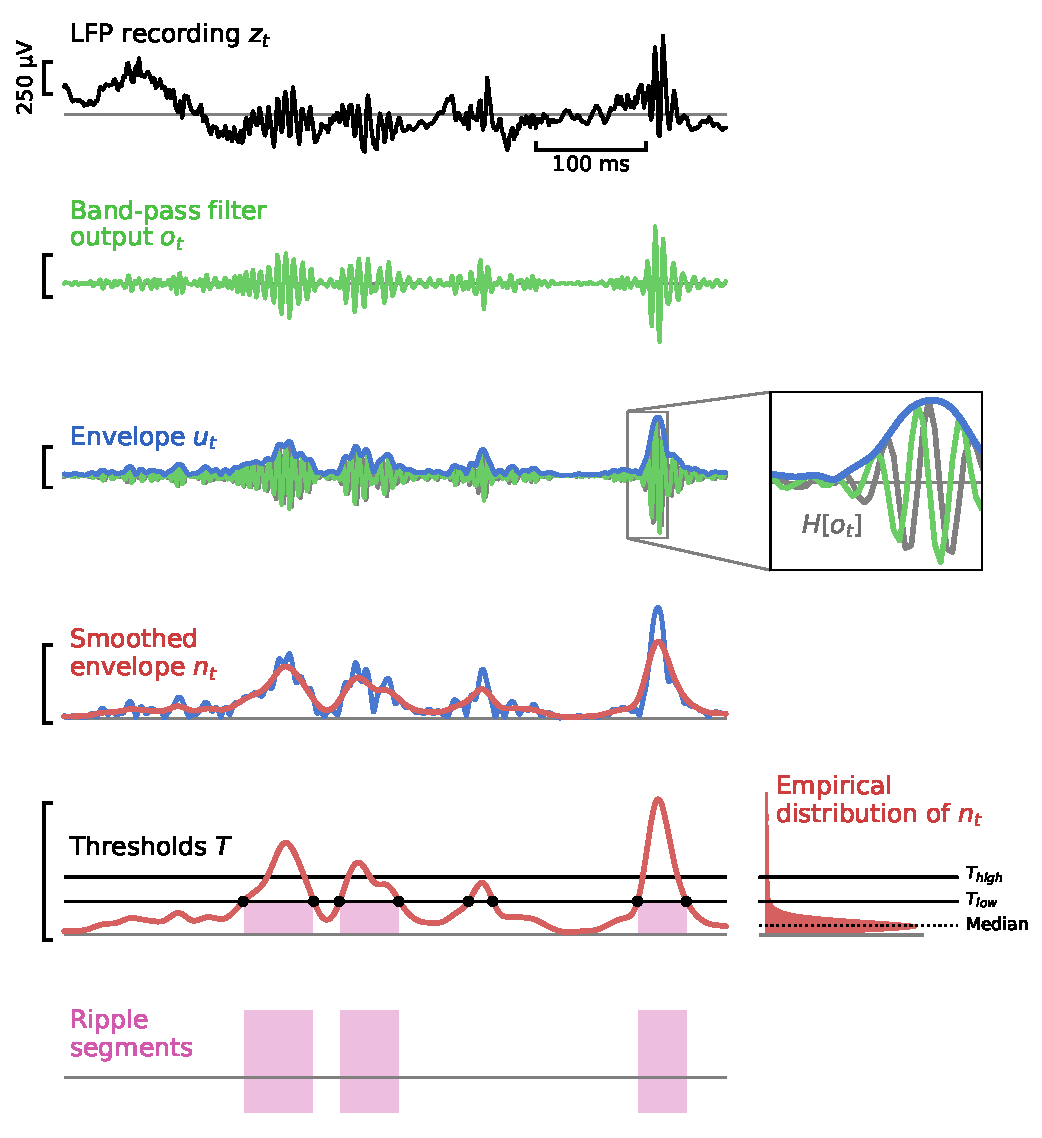
\includegraphics{figures/107_2--107_8}
\captionn{Steps for automated, offline SWR labelling}{See text for details. Each vertical scalebar indicates the same voltage range. $H[o_t]$ denotes the Hilbert transform of $o_t$. Note its phase lag of 90\si{\degree} with respect to $o_t$. In the second panel from the bottom, note the two threshold crossings of $T\low$ (marked with black dots) that did not result in a ripple segment, because the second threshold $T\high$ was not reached. The distribution of the envelope $n_t$ was estimated using the entire dataset (and not just the displayed time slice).}
\label{fig:offline-steps}
\end{figure}


The following few subsections describe these detection steps in more detail, and compare our method and parameter choices with those made in the literature.

If not mentioned otherwise, our parameter choices were made as follows:
In a first pass of the offline detection algorithm, ripples were detected using a very broad-band filter and a low detection threshold. This ensured that all `true' SWR's were included in the detected events set (in addition to many spurious detections).

Next, five neuroscientists were independently asked to decide for each detected event whether it was an SWR event or not. (This was done through a custom-made web app, an example view of which is depicted in \cref{fig:labelface-UI}). Only the events that were labelled as an SWR by at least three neuroscientists were retained.

Lastly, when setting a parameter of the final offline ripple detection algorithm, the algorithm's output was compared with the decisions made by the neuroscientists. The parameter was then adjusted until the output of the algorithm matched the neuroscientist decisions reasonably well.



\subsection{Band-pass filter}

The wideband voltage signal $x_t$ was band-pass filtered between 100 and 200 Hz, using a linear, time-invariant filter with zero output lag. The frequency band was chosen based on t



\subsection{Envelope}



\subsection{Thresholds}



% Decision: 
% - details in text, or in figure.
% - put numbers in figure caption, see if it works, if not, move to text.
% What is it?
% - smoothing kernel & bw
% - Hilbert transform, it's magnitude, kernel, and phase shift effect
% - bandpass filter type, band, order, freq response, zero-lag
% - 

% standardized data
